%\documentclass[letterpaper]{amsart}
\documentclass[letterpaper]{tufte-handout}
\usepackage{times}
\usepackage{amsmath}
\usepackage{amssymb}
\usepackage{graphicx}
\usepackage{booktabs}
\usepackage{multirow}
\usepackage{listings}
\usepackage{epstopdf}
\usepackage{bm}
\usepackage{natbib}
%\usepackage[left=1in]{geometry}

\newcommand{\R}{\mathcal{R}}
\newcommand{\E}{\text{E}}
\newcommand{\p}{p_{XY}}
\newcommand{\T}{^\text{T}}
\newcommand{\y}{\mathbf{y}}
\newcommand{\z}{\mathbf{z}}
\newcommand{\I}{\mathbf{I}}
\newcommand{\HH}{\mathbf{H}}
\newcommand{\A}{\mathbf{A}}
\newcommand{\GG}{\mathbf{G}}
\newcommand{\vecv}{\mathbf{v}}
\newcommand{\uu}{\mathbf{u}}
\newcommand{\cyy}{\mathbf{C}_{yy}}
\newcommand{\cyz}{\mathbf{C}_{yz}}
\newcommand{\czz}{\mathbf{C}_{zz}}
\newcommand{\cuu}{\mathbf{C}_{uu}}
\newcommand{\cvv}{\mathbf{C}_{vv}}
\newcommand{\cpp}{\mathbf{C}_{\psi\psi}}
\renewcommand{\arraystretch}{1.5}
\newcommand{\KK}{\left(\begin{array}{c} \frac{{\sigma_{\y_1}}^2}{{\sigma_v}^2 + {\sigma_{\y_1}}^2}\\ \frac{\sigma_{\y_1\y_2}}{{\sigma_v}^2 + {\sigma_{\y_1}}^2} \end{array}\right)}
\newcommand{\cyylong}{\left(\begin{array}{cc} {\sigma_{y_1}}^2 & \sigma_{\y_1\y_2}\\ \sigma_{\y_1\y_2} & {\sigma_{y_2}}^2 \end{array}\right)}
  \renewcommand{\vec}[1]{\mathrm{#1}}

  \title{Problem Set 8 --- ENCE689E Spring 2014}
  \author{David Prentiss}

  \begin{document}
  \maketitle

  \section{1. Precipitation Errors}
  \subsection{(a)} 
  See Figure \ref{1a} and Listing \ref{list1b}.
  \begin{figure}
    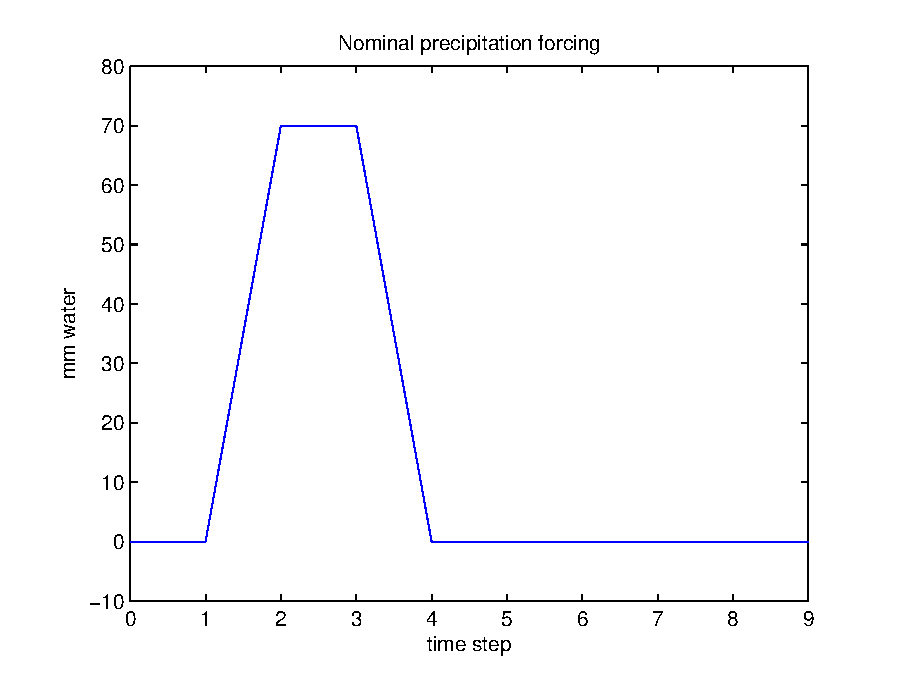
\includegraphics[width=\textwidth]{1a}
    \caption{Nominal precipitation forcing from Problem Set 5.}
    \label{1a}
  \end{figure}
  \subsection{(b)}
  \begin{itemize}
    \item For the unbiasedness assumption, the mean of the additive error must be zero.
    \item A ten--member ensemble was generated with the code in Listing \ref{list1b} and plotted in Figure 2. 

    \item The variance of the error term was chosen to be $\sigma^2_u = 1$. This value implies that approximately 95\% of the forcing are within 2 standard deviations (2mm) of the nominal forcing and, by implication, within that same range of the true value. 
    \item Because it is unlikely that readings from a rain gauge would underestimate the precipitation during a period when the true value is zero, we should question the assumption that the error is unbiased.
      This is especially true of a gauge that can not (or practically does not) indicate negative values. Furthermore, while it is certainly possible to underestimate positive precipitation amounts, this lack of "negative" error should cause us to question the Gaussian assumption as well, even if we postulate a positive bias.
    \item Even if the forcing error may be appropriately considered Gaussian, it relationship with the model is nonlinear and therefore, introduce non-Gaussian error in the model.
  \end{itemize}
  {\small
    \lstinputlisting[language=Matlab, caption={Ten--memeber, precipitation forcing ensemble.},
    basicstyle=\ttfamily, label=list1b]{ps8_1.m}
  }
  \begin{figure}
    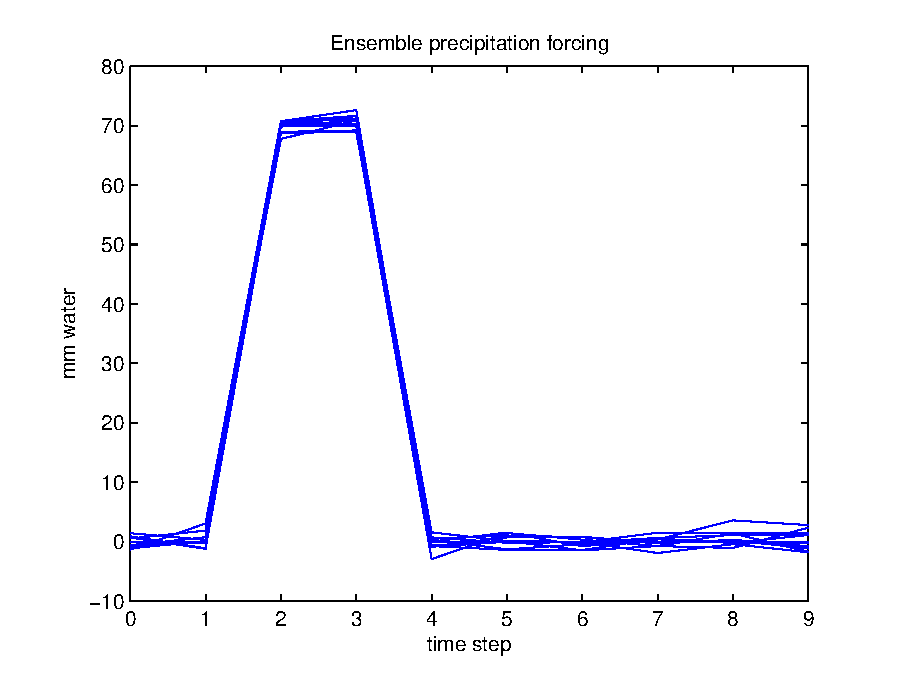
\includegraphics[width=\textwidth]{1b}
    \caption{Nominal precipitation forcing from Problem Set 5.}
    \label{1b}
  \end{figure}
  \subsection{(c)}
  \begin{itemize}
    \item See Listing \ref{list1b} and Figure \ref{1c}
  \end{itemize}
  \subsection{(d)}
  \begin{itemize}
    \item The primary benefit of of using multiplicative error is the possibility of eliminating negative values from the precipitation.
    \item The mean of the multiplicative error must be one (1) to ensure the ensemble is unbiased.
  \end{itemize}
  \subsection{(e)}
  \begin{itemize}
    \item See Listing \ref{list1b} and Figure \ref{1e}
  \end{itemize}
  \subsection{(f)}
  \begin{itemize}
    \item See Listing \ref{list1b} and Figure \ref{1f}
  \end{itemize}
  \subsection{(g)}
  \section{2. Parameter Estimation}
  \begin{itemize}
    \item For the prior parameter distribution, we can truncate and double the negative side of the normal distribution. That is, if $X$ is any zero mean, Gaussian distribution, we will assume $u = -|X|$. There many distributions that would suffice to eliminate positive values, however this one has the advantage of easy implementation for Monte Carlo methods.
    \item Eliminating positive predictions and updates was accomplished by overwriting any positive values for the parameter estimation state with its multiplicative opposite. For example, line 3 in the code below was added to the loop.
      \begin{verbatim}
   for k = 1:Nreps
       Y0(1:length(Ybar),k) = mvnrnd(Ybar,Cy0y0,1)';
       Y0(3,k) = -abs(Y0(3,k));
       zz(1,1,k) = H*Y0(:,k);
   end
   \end{verbatim}
 \item The change of prior distribution had the following effect on the performance of the EnKF and open-loop models:
   \begin{table}
     \begin{tabular}{llll}
       & Original Prior & Improved Prior & Open Loop \\
       RMSE & 2.1846 & 1.9632 & 2.5949 \\
       Bias & 0.5834 & 0.4489 & 0.771
     \end{tabular}
   \end{table}
 \item See listing 2.
\end{itemize}
{\small
  \lstinputlisting[language=Matlab, caption={Parameter Prior Distribution Performance Calculations},
  basicstyle=\ttfamily, label=list2]{ps8_2.m}
}
\section{3. Spatially-Homogeneous Force-Restore Model with the EnKF}
\subsection{(a)}
\begin{itemize}
\item The state vector is \[y = \begin{pmatrix} y_1 \\ y_2 \\ y_3 \\ y_4 \end{pmatrix}\]
  \item The measurement model is \[H = [0\ 0\ 1\ 0]\].
  \item measurement error
  \item mean
  \item covariance 
  \item true precipitation error
\end{itemize}
\subsection{(b)}
\begin{figure}
  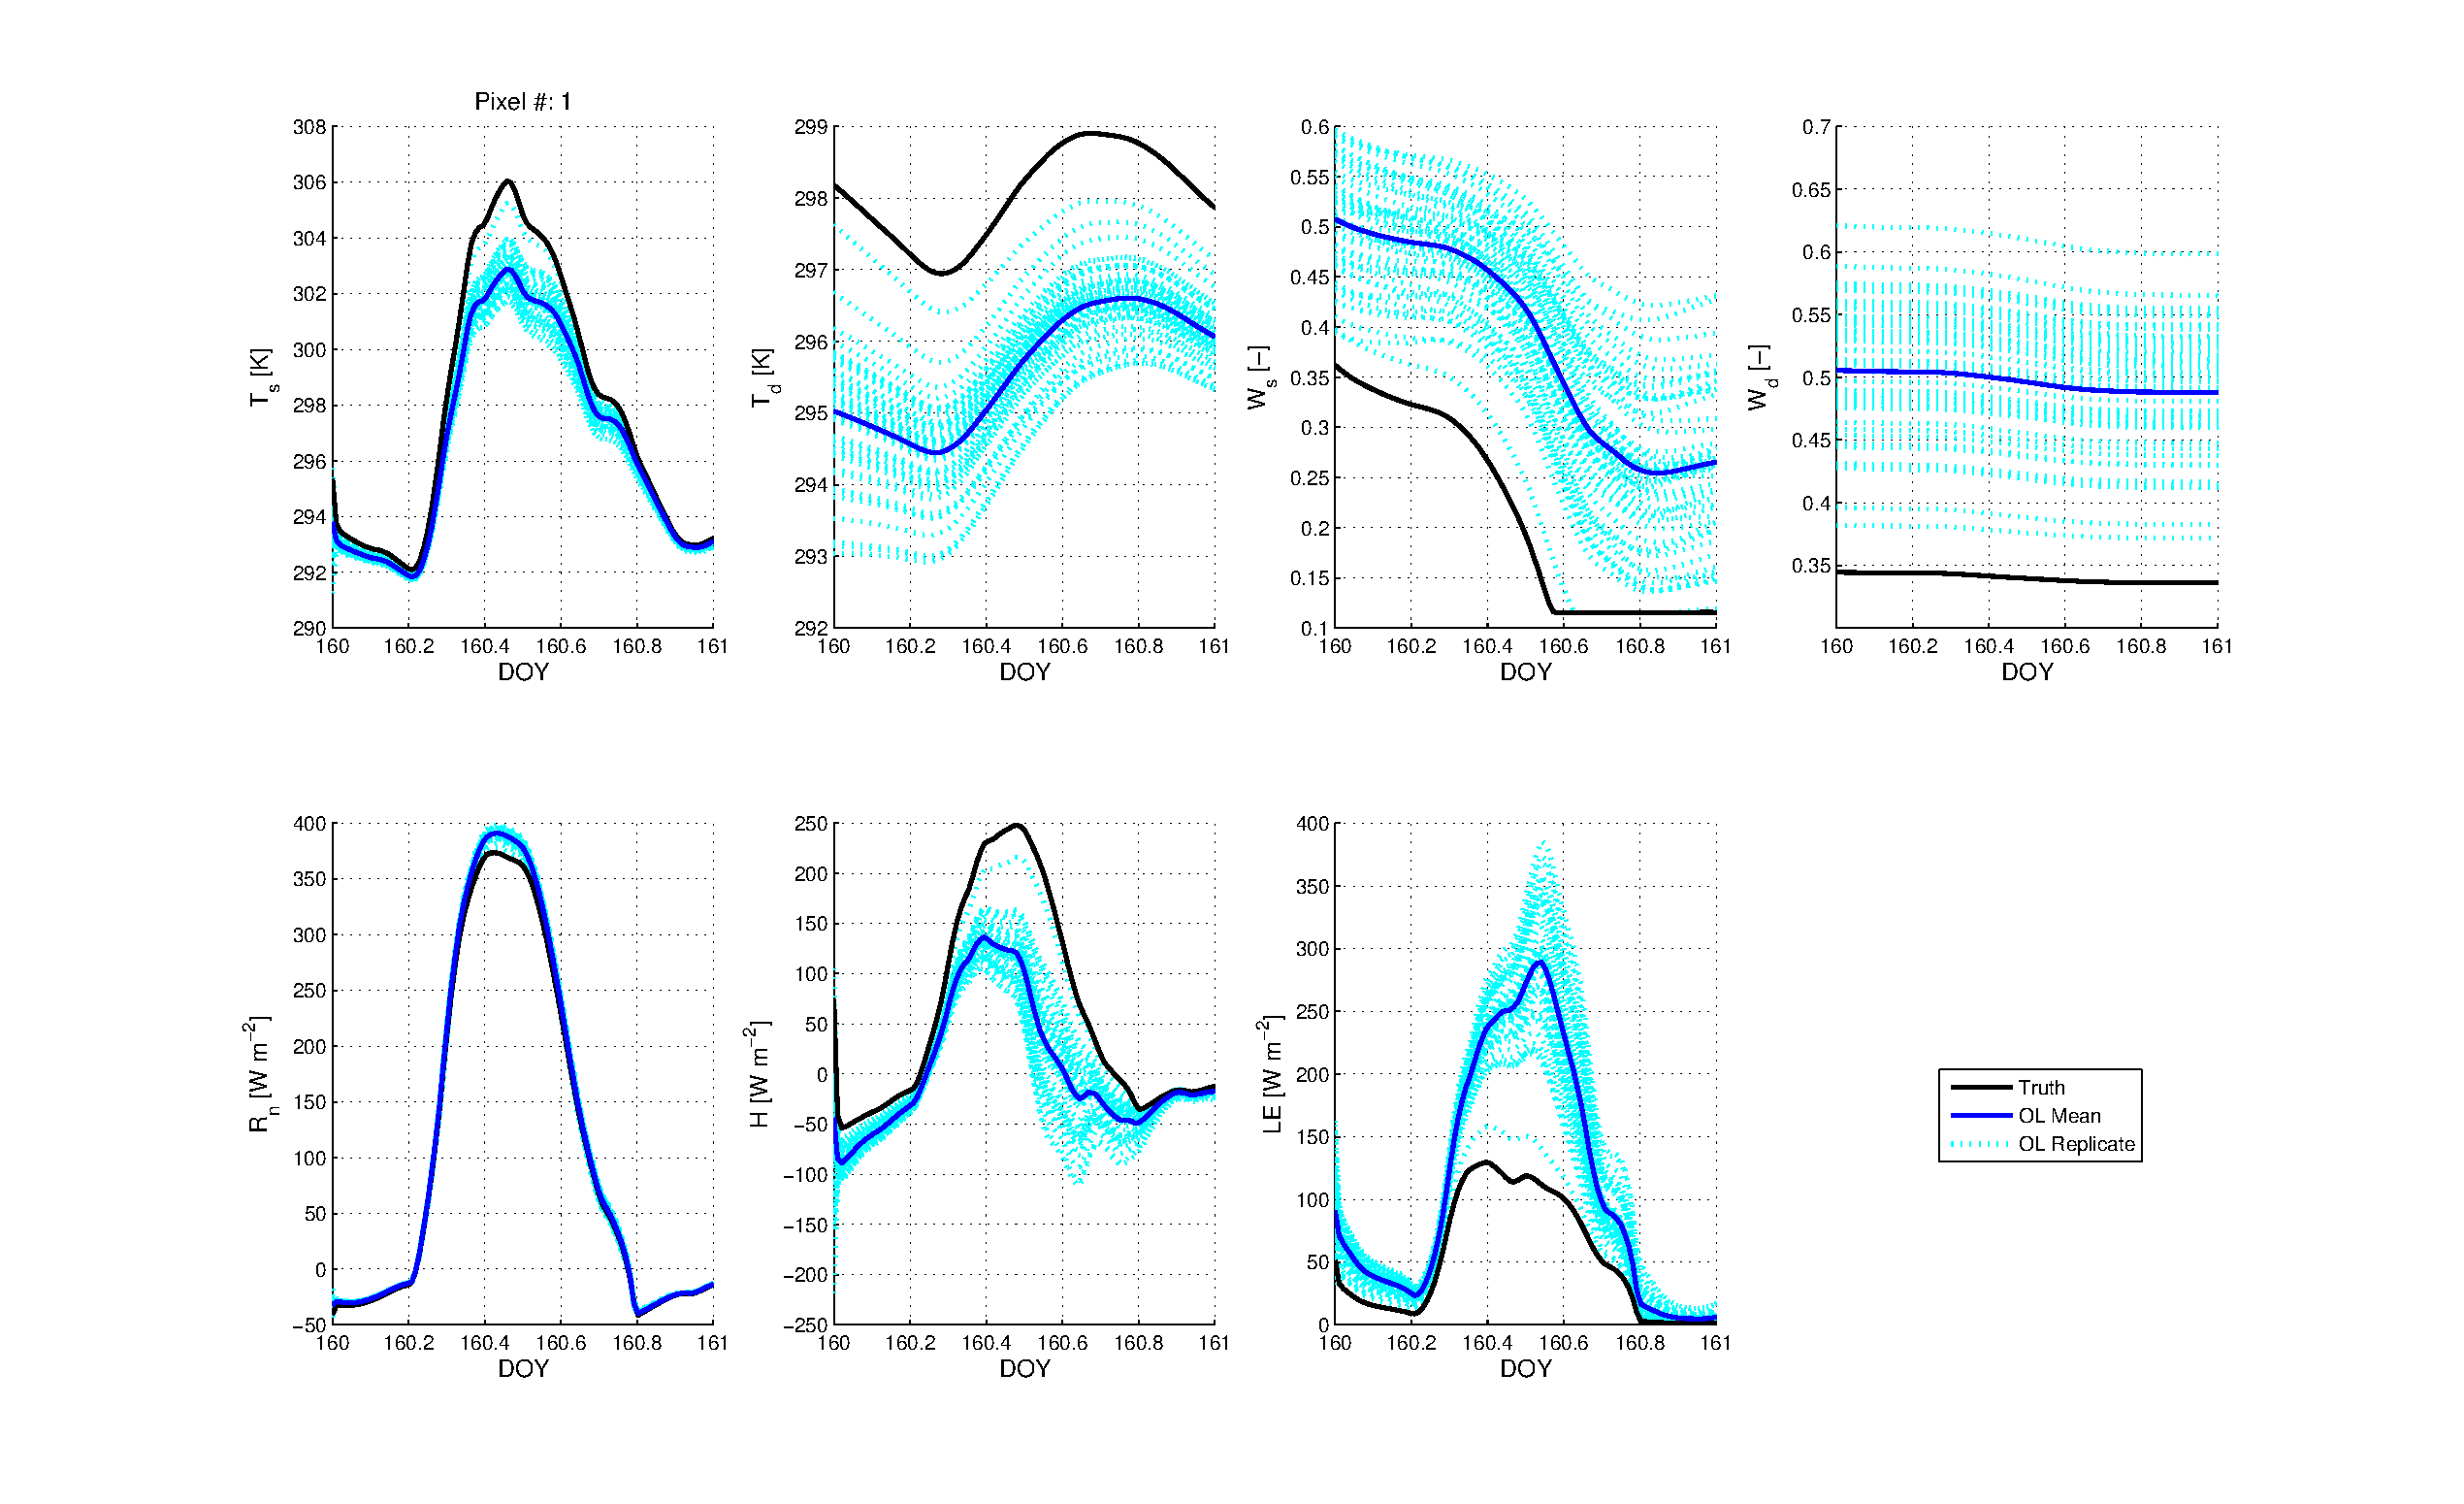
\includegraphics[width=\textwidth]{3b}
  \caption{}
\end{figure}
\subsection{(c)}
{\small
  \lstinputlisting[language=Matlab, caption={Parameter Prior Distribution Performance Calculations},
  basicstyle=\ttfamily, label=list2]{ps8_2.m}
}
\begin{figure}
  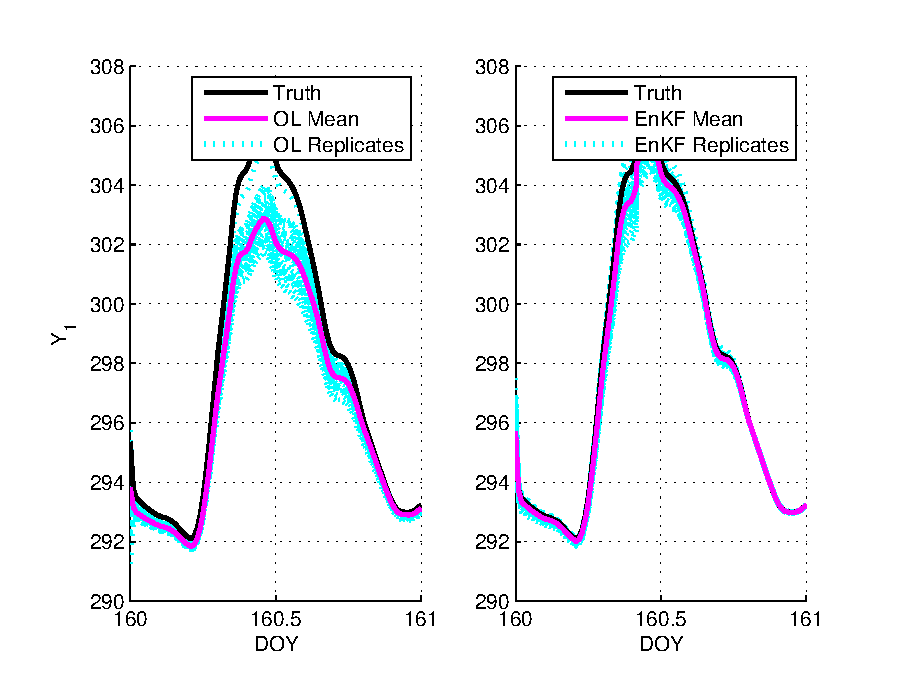
\includegraphics[width=\textwidth]{3cy1}
  \caption{}
\end{figure}
\begin{figure}
  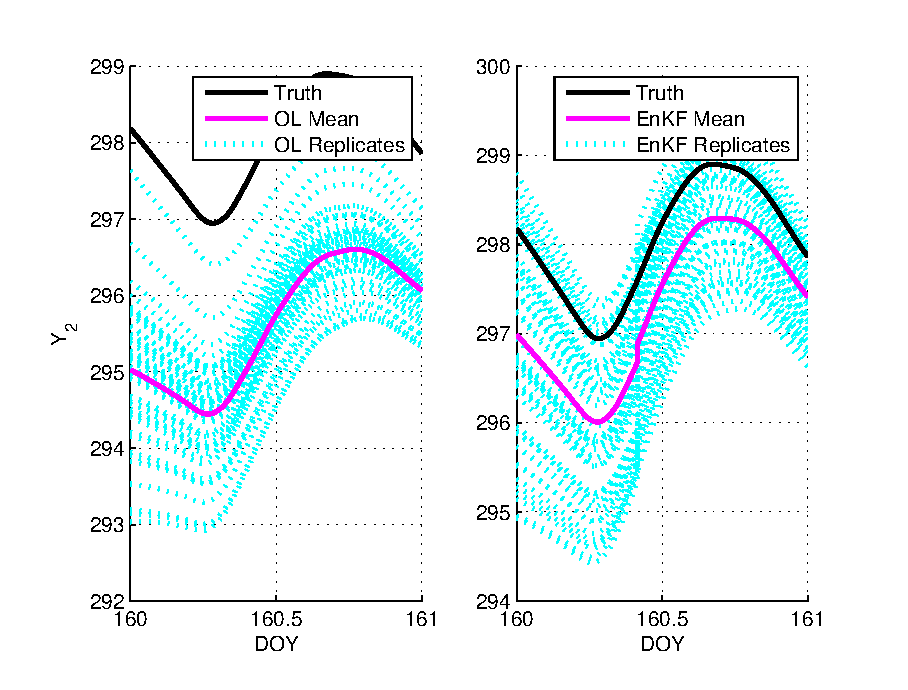
\includegraphics[width=\textwidth]{3cy2}
  \caption{}
\end{figure}
\begin{figure}
  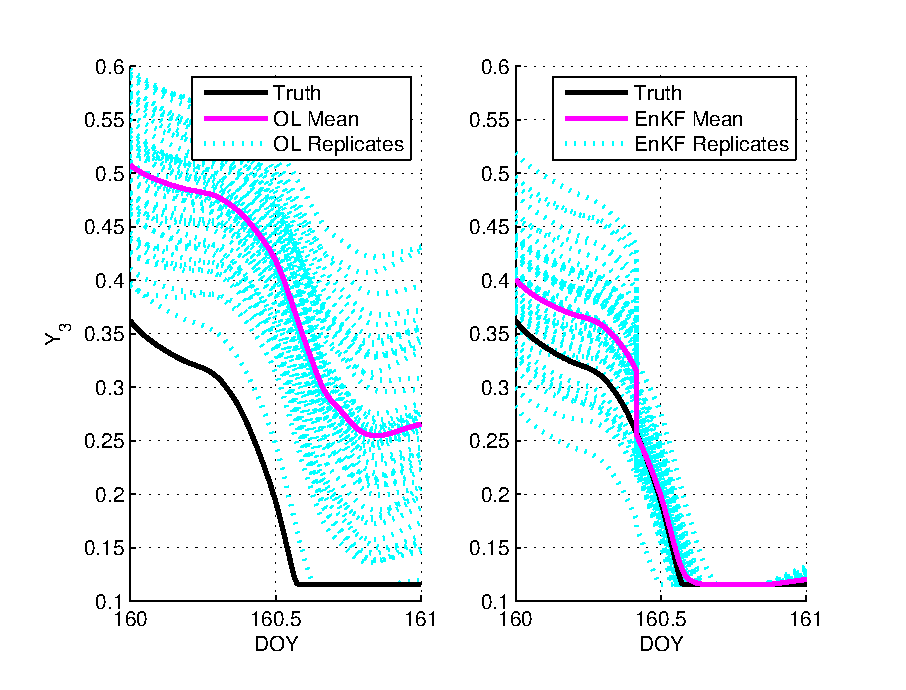
\includegraphics[width=\textwidth]{3cy3}
  \caption{}
\end{figure}
\begin{figure}
  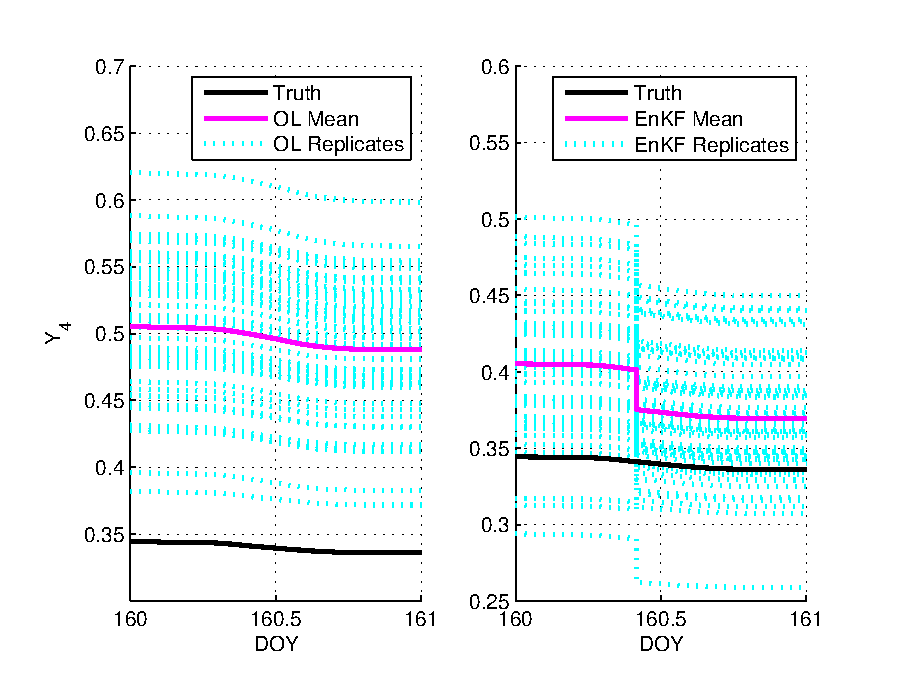
\includegraphics[width=\textwidth]{3cy4}
  \caption{}
\end{figure}
\begin{figure}
  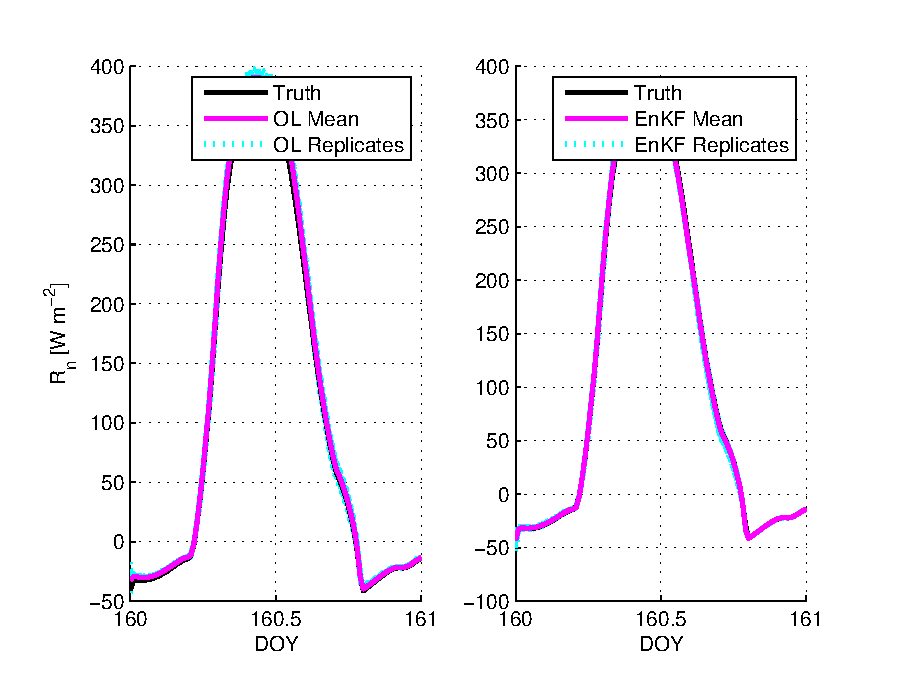
\includegraphics[width=\textwidth]{3cr}
  \caption{}
\end{figure}
\begin{figure}
  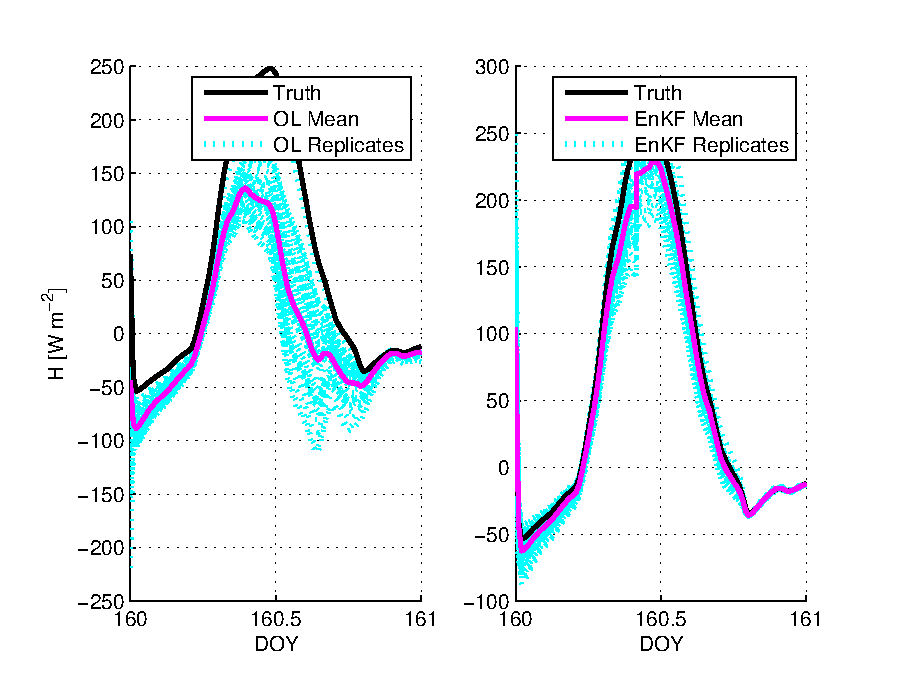
\includegraphics[width=\textwidth]{3ch}
  \caption{}
\end{figure}
\begin{figure}
  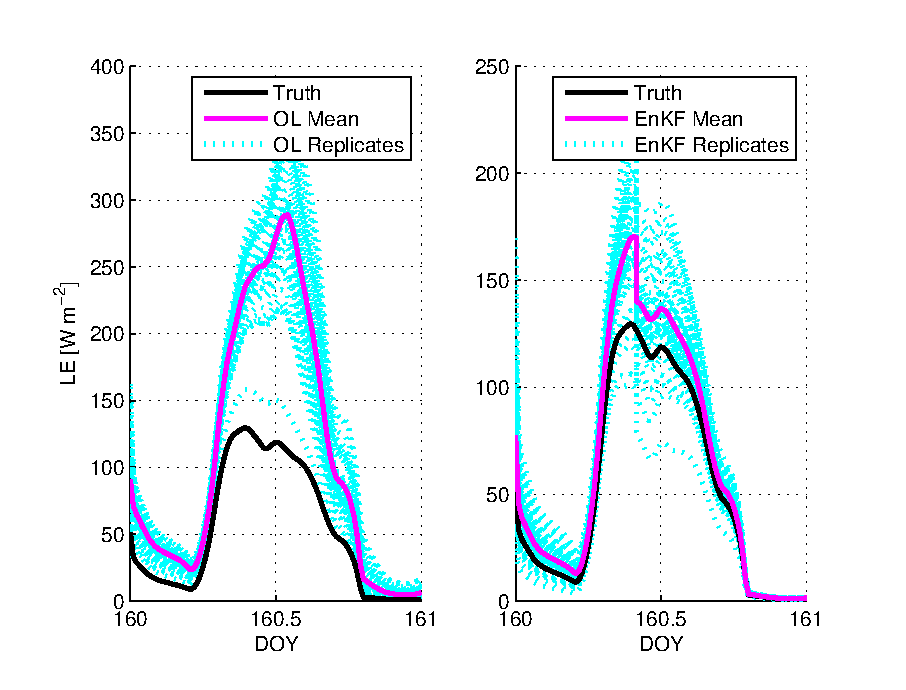
\includegraphics[width=\textwidth]{3cle}
  \caption{}
\end{figure}
\begin{table}
  \begin{tabular}{rccccccc} 
    &$T_s$ & $T_d$ & $W_s$ & $W_d$ & $R_n$ & $H$ & $LE$ \\
    RMSE & 0.3417 & 0.7995 & 0.02976 & 0.0467 & 2.372 & 14.12 & 13.87\\
    Bias & -0.2174 & -0.7669 & 0.02032 & 0.04477 & -0.05925 & -9.922 & 10.14
  \end{tabular}
\end{table}

\subsection{(d)}
{\small
  \lstinputlisting[language=Matlab, caption={ps8\_3d},
  basicstyle=\ttfamily, label=list2]{ps8_3d.m}
}
From the resulting covariance matrix
\[\left(\begin{array}{cccc} 0.005845 & 0.01838 & -0.005506 & -0.002752\\ 0.01838 & 0.1536 & -0.01681 & -0.009814\\ -0.005506 & -0.01681 & 0.005577 & 0.002721\\ -0.002752 & -0.009814 & 0.002721 & 0.002458 \end{array}\right)\],
the correlation matrix
\[\left(\begin{array}{cccc} 1.0 & 0.6135 & -0.9644 & -0.726\\ 0.6135 & 1.0 & -0.5745 & -0.505\\ -0.9644 & -0.5745 & 1.0 & 0.735\\ -0.726 & -0.505 & 0.735 & 1.0 \end{array}\right)\],
and the relationship
\[\text{Cov}[X,Y] = \rho_{xy}\sigma_x\sigma_y\]
we can calculate a new initial covariance matrix


\subsection{(e)} This is an improvement over the results is section 3c.

\begin{table}
  \begin{tabular}{rccccccc} 
    &$T_s$ & $T_d$ & $W_s$ & $W_d$ & $R_n$ & $H$ & $LE$ \\
    RMSE &0.1433 & 0.3029 & 0.03139 & 0.01868 & 3.215 & 6.684 & 8.09\\
    Bias &0.03261 & -0.246 & -0.02033 & 0.01384 & -1.551 & 2.057 & -3.331
  \end{tabular}
\end{table}

\section{4. Spatially-Distributed Force-Restore Model with the EnKF}
\subsection{(a)}
\begin{itemize}
  \item The state vector is \[y =
      \begin{pmatrix} y_{1,1} \\ y_{2,1} \\ y_{3,1} \\ y_{4,1} \\
        y_{1,2} \\ y_{2,2} \\ y_{3,2} \\ y_{4,2} \\
        y_{1,3} \\ y_{2,3} \\ y_{3,3} \\ y_{4,3} \\
        y_{1,4} \\ y_{2,4} \\ y_{3,4} \\ y_{4,4} \\
    \end{pmatrix}\]
  \item The measurement model is \[H = [0\ 0\ 1\ 0]\].
\end{itemize}
\subsection{(b)}
\begin{figure}
  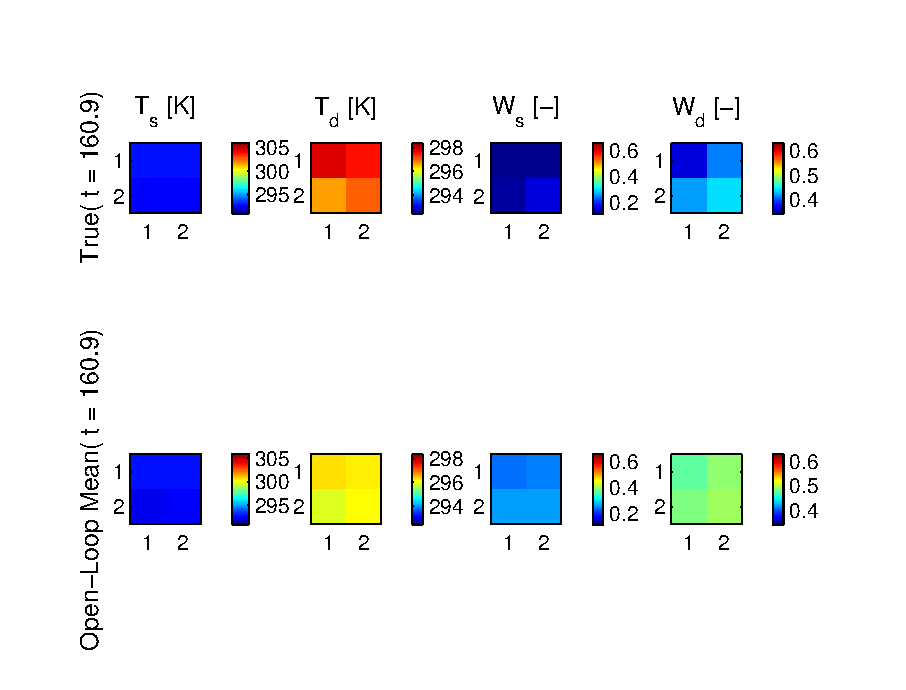
\includegraphics[width=\textwidth]{4b1map}
  \caption{}
\end{figure}
\begin{figure}
  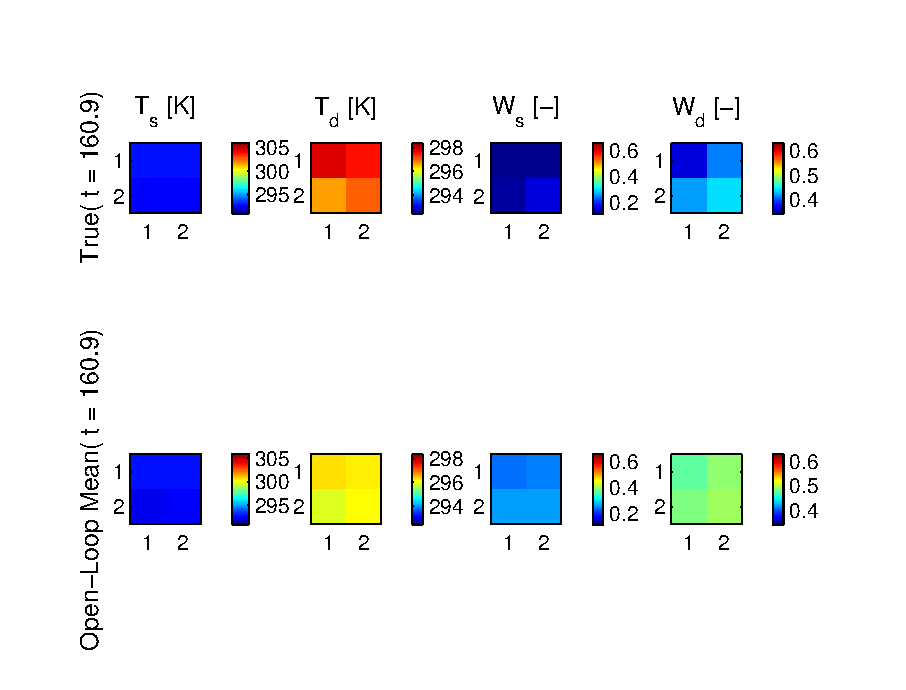
\includegraphics[width=\textwidth]{4b4map}
\end{figure}
\begin{figure}
  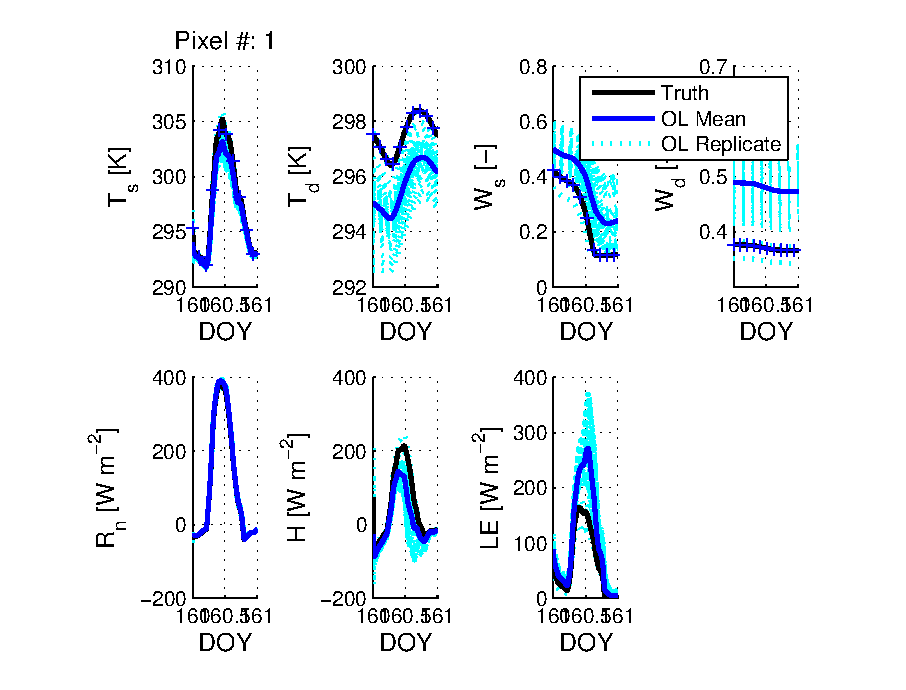
\includegraphics[width=\textwidth]{4b1ts}
\end{figure}
\begin{figure}
  \includegraphics[width=\textwidth]{4b41ts}
\end{figure}
\subsection{(c)}
\begin{figure}
  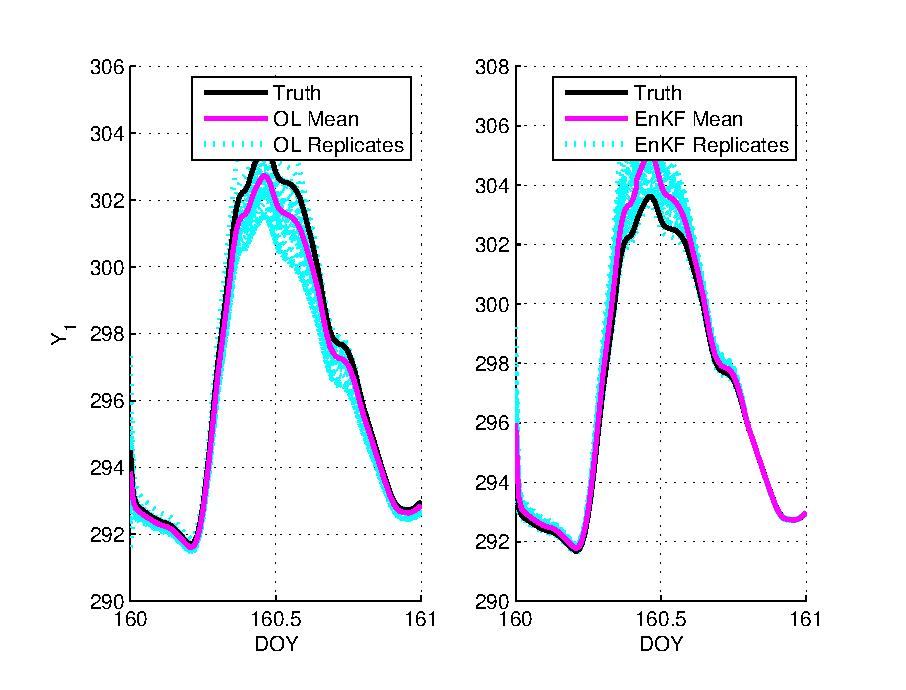
\includegraphics[width=\textwidth]{4cy1}
  \caption{}
\end{figure}
\begin{figure}
  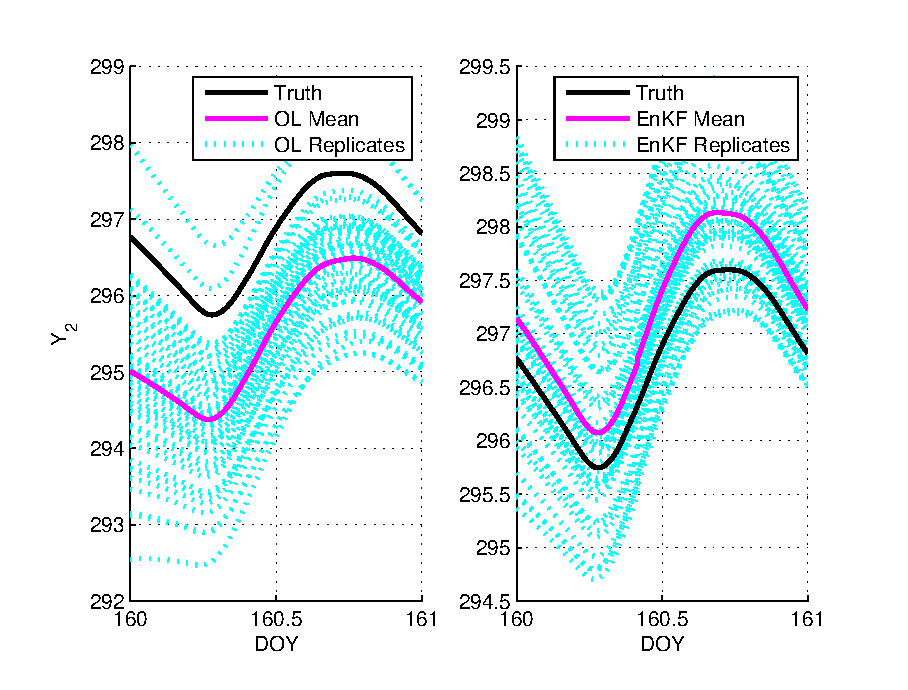
\includegraphics[width=\textwidth]{4cy2}
  \caption{}
\end{figure}
\begin{figure}
  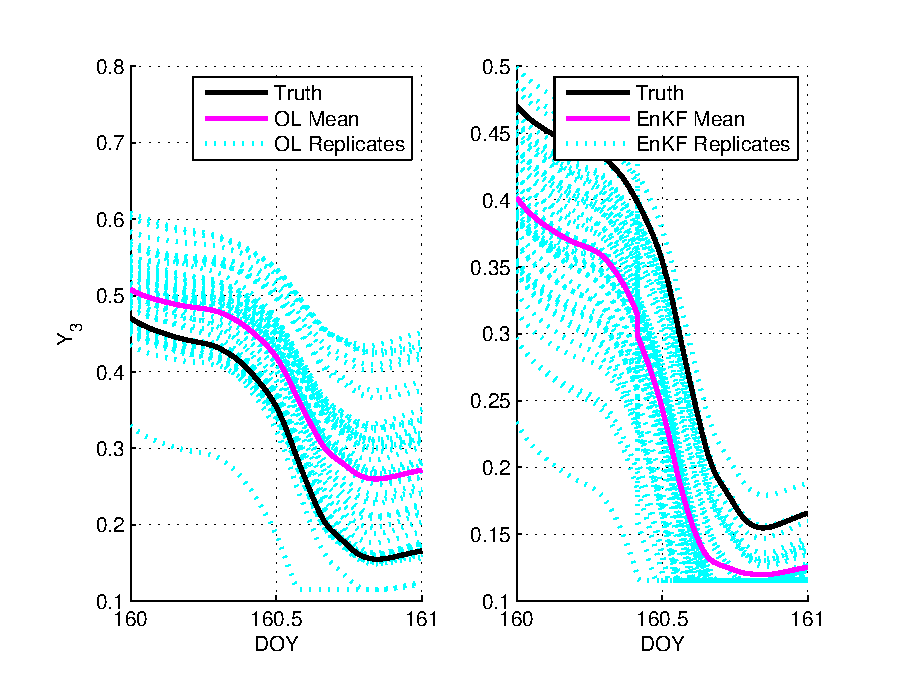
\includegraphics[width=\textwidth]{4cy3}
  \caption{}
\end{figure}
\begin{figure}
  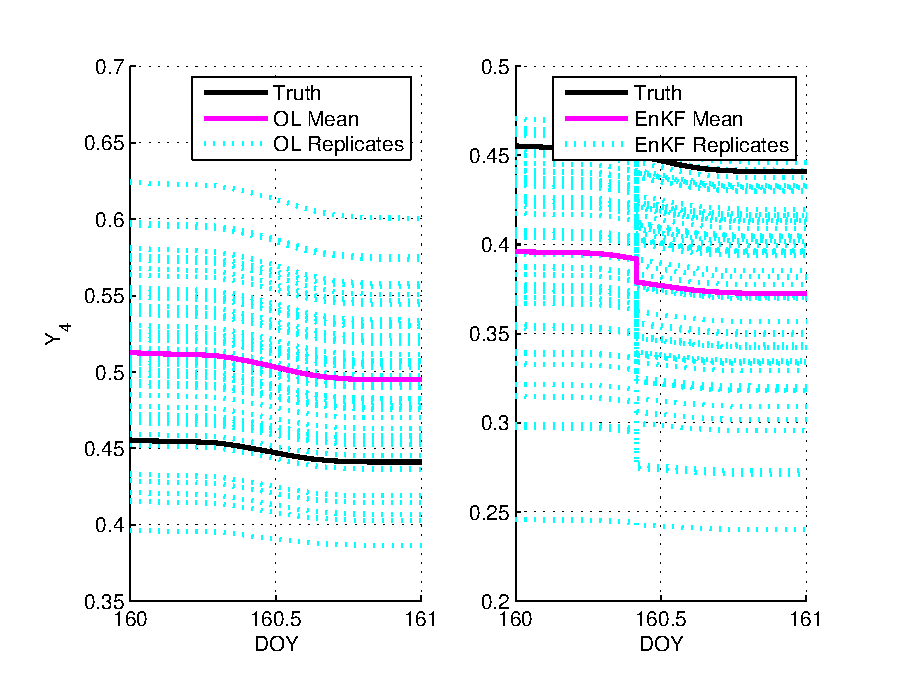
\includegraphics[width=\textwidth]{4cy4}
  \caption{}
\end{figure}
\begin{figure}
  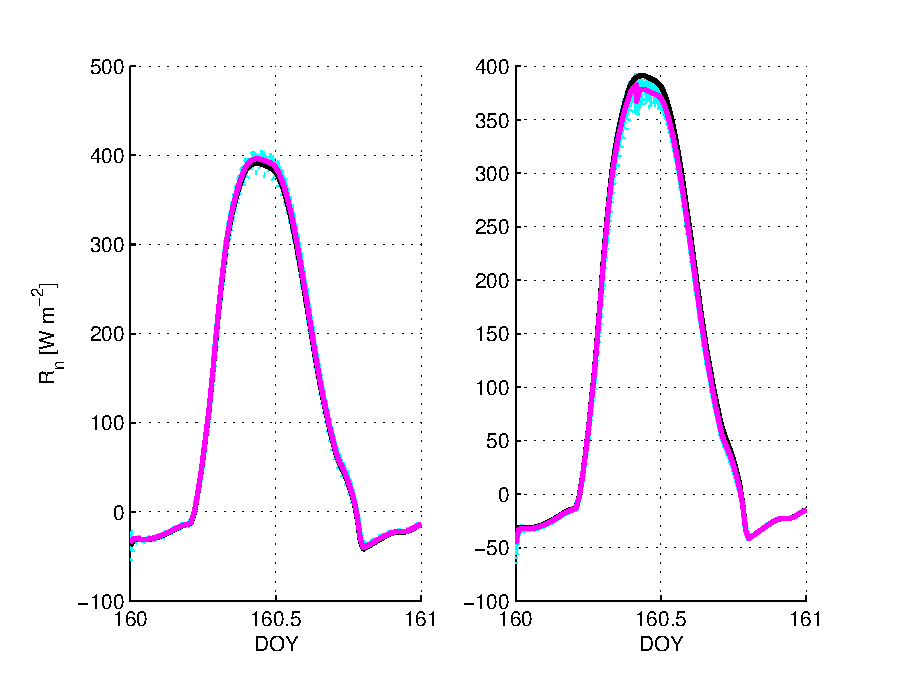
\includegraphics[width=\textwidth]{4cr}
  \caption{}
\end{figure}
\begin{figure}
  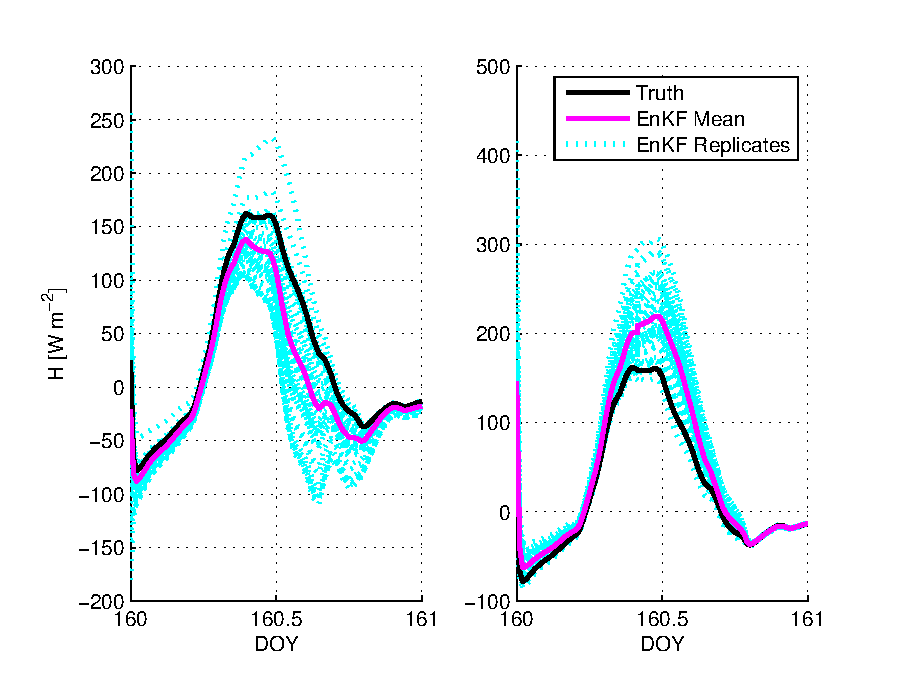
\includegraphics[width=\textwidth]{4ch}
  \caption{}
\end{figure}
\begin{figure}
  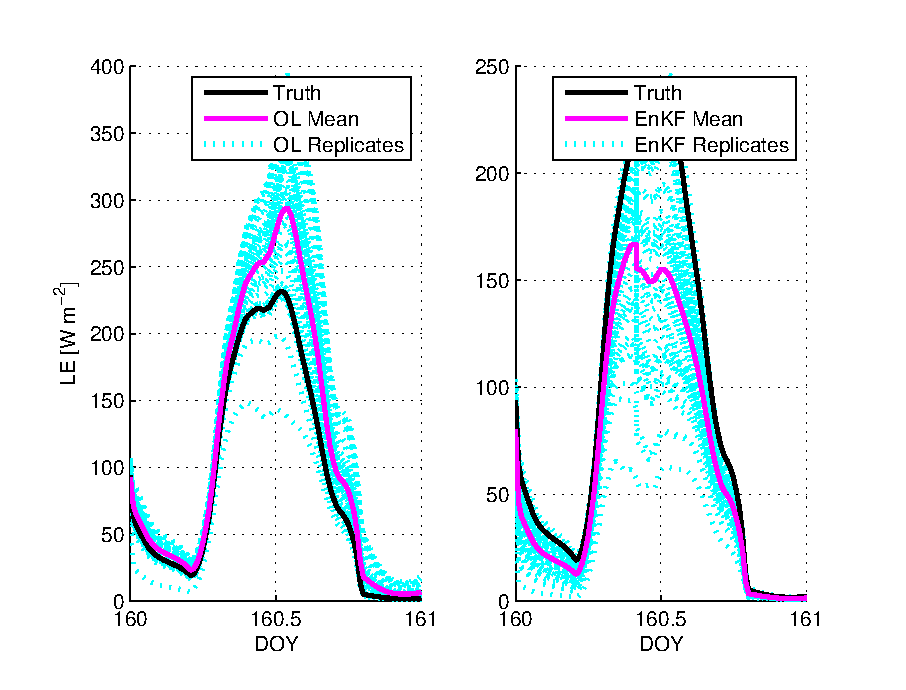
\includegraphics[width=\textwidth]{4cle}
  \caption{}
\end{figure}
\subsection{(d)}
{\small
  \lstinputlisting[language=Matlab, caption={ps8\_4d.m},
  basicstyle=\ttfamily, label=list2]{ps8_4d.m}
}
\begin{table}
  \begin{tabular}{rccccccc} 
    &$T_s$ & $T_d$ & $W_s$ & $W_d$ & $R_n$ & $H$ & $LE$ \\
    RMSE, px 1 & 0.1488 & 0.3615 & 0.01214 & 0.03153 & 2.722 & 8.56 & 5.201\\
    Bias, px 1 & -0.08062 & -0.3383 & -0.00273 & 0.03037 & -1.323 & -3.806 & 2.904\\
    RMSE, px 2 &0.2038 & 0.6563 & 0.02195 & 0.02549 & 1.866 & 11.31 & 10.41\\
    Bias, px 2 &0.1457 & 0.6469 & -0.01714 & -0.0253 & -0.2465 & 7.831 & -6.948\\
    RMSE, px 3 &0.1723 & 0.2011 & 0.00857 & 0.03299 & 1.159 & 9.433 & 9.861\\
    Bias, px 3 &0.1066 & -0.1325 & -0.002256 & -0.03254 & -0.2915 & 5.706 & -6.189\\
    RMSE, px 4 &0.6304 & 0.4457 & 0.07474 & 0.06493 & 6.39 & 32.01 & 34.71\\
    Bias, px 4 & 0.4249 & 0.4382 & -0.07083 & -0.06474 & -4.409 & 21.71 & -24.56 
  \end{tabular}
\end{table}

\end{document}
